\documentclass[openany]{book}

\usepackage[margin=1in]{geometry}
\usepackage{amsmath,amsfonts,amsthm, amssymb}
\usepackage{yhmath}
\usepackage{mathrsfs}
\usepackage{mathtools}
\usepackage{xcolor}
\usepackage{graphicx}
\usepackage{tikz-cd}
\usepackage{comment}
\renewcommand{\familydefault}{ppl}
\newcommand{\R}{\mathbb{R}}
\newcommand{\E}{\mathbb{E}}
\newcommand{\Z}{\mathbb{Z}}
\newcommand{\Q}{\mathbb{Q}}
\newcommand{\C}{\mathbb{C}}
\let\oldemptyset\emptyset
\let\emptyset\varnothing

\let\oldepsilon\epsilon
\let\epsilon\varepsilon

\usepackage{thmtools,thm-restate}

% Fixing mdframed skip below
% See https://tex.stackexchange.com/a/292090/143086
\usepackage[framemethod=TikZ]{mdframed}
\usepackage{xpatch}
\makeatletter
\xpatchcmd{\endmdframed}
	{\aftergroup\endmdf@trivlist\color@endgroup}
	{\endmdf@trivlist\color@endgroup\@doendpe}
	{}{}
\makeatother

\definecolor{huilightpink}{HTML}{fff2fe}
\definecolor{huidarkpink}{HTML}{d955b7}
\declaretheoremstyle[
	mdframed={
		backgroundcolor=huilightpink,
		linecolor=huidarkpink,
		rightline=false,
		topline=false,
		bottomline=false,
		linewidth=2pt,
		innertopmargin=5pt,
		innerbottommargin=8pt,
		innerleftmargin=8pt,
		leftmargin=-2pt,
		skipbelow=2pt,
		nobreak
	},
	headfont=\normalfont\bfseries\color{huidarkpink}
]{huipinkbox}
\declaretheorem[style=huipinkbox,name=Theorem,within=chapter]{thm}
\declaretheorem[style=huipinkbox,name=Theorem,sibling=thm]{theorem}




\begin{comment}
\definecolor{huilightyellow}{HTML}{fff5d6}
\definecolor{huidarkyellow}{HTML}{fcad03}
\declaretheoremstyle[
	mdframed={
		backgroundcolor=huilightyellow,
		linecolor=huidarkyellow,
		rightline=false,
		topline=false,
		bottomline=false,
		linewidth=2pt,
		innertopmargin=5pt,
		innerbottommargin=8pt,
		innerleftmargin=8pt,
		leftmargin=-2pt,
		skipbelow=2pt,
		nobreak
	},
	headfont=\normalfont\bfseries\color{huidarkyellow}
]{huiyellowbox}
\declaretheorem[style=huiyellowbox,name=Proposition,within=chapter]{prop}
\end{comment}



\definecolor{huilightpurple}{HTML}{faf2ff}
\definecolor{huidarkpurple}{HTML}{912ed9}
\declaretheoremstyle[
	mdframed={
		backgroundcolor=huilightpurple,
		linecolor=huidarkpurple,
		rightline=false,
		topline=false,
		bottomline=false,
		linewidth=2pt,
		innertopmargin=5pt,
		innerbottommargin=8pt,
		innerleftmargin=8pt,
		leftmargin=-2pt,
		skipbelow=2pt,
		nobreak
	},
	headfont=\normalfont\bfseries\color{huidarkpurple}
]{huipurplebox}
\declaretheorem[style=huipurplebox,name=Proposition,within=chapter]{prop}



% \definecolor{huilightpurple}{HTML}{faf2ff}
% \definecolor{huidarkpurple}{HTML}{912ed9}
% \declaretheoremstyle[
% 	mdframed={
% 		backgroundcolor=huilightpurple,
% 		linecolor=huidarkpurple,
% 		rightline=false,
% 		topline=false,
% 		bottomline=false,
% 		linewidth=2pt,
% 		innertopmargin=5pt,
% 		innerbottommargin=8pt,
% 		innerleftmargin=8pt,
% 		leftmargin=-2pt,
% 		skipbelow=2pt,
% 		nobreak
% 	},
% 	headfont=\normalfont\bfseries\color{huidarkpurple}
% ]{huipurplebox}
\declaretheorem[style=huipurplebox,name=Lemma,within=chapter]{lem}


\definecolor{lightpink}{HTML}{f0f6fc}
\definecolor{darkpink}{HTML}{2c72b8}
\declaretheoremstyle[
	mdframed={
		backgroundcolor=lightpink,
		linecolor=darkpink,
		rightline=false,
		topline=false,
		bottomline=false,
		linewidth=2pt,
		innertopmargin=5pt,
		innerbottommargin=8pt,
		innerleftmargin=8pt,
		leftmargin=-2pt,
		skipbelow=2pt,
		nobreak
	},
	headfont=\normalfont\bfseries\color{darkpink}
]{pinkbox}
\declaretheorem[style=pinkbox,name=Definition,within=chapter]{defn}


\definecolor{huilightblue}{HTML}{edf9ff}
\definecolor{huidarkblue}{HTML}{4b79db}
\declaretheoremstyle[
	mdframed={
		backgroundcolor=huilightblue,
		linecolor=huidarkblue,
		rightline=false,
		topline=false,
		bottomline=false,
		linewidth=2pt,
		innertopmargin=5pt,
		innerbottommargin=8pt,
		innerleftmargin=8pt,
		leftmargin=-2pt,
		skipbelow=2pt,
		nobreak
	},
	headfont=\normalfont\bfseries\color{huidarkblue}
]{huiblueblox}
\declaretheorem[style=huiblueblox,name=Example,within=chapter]{example}



% \definecolor{huilightblue}{HTML}{edf9ff}
% \definecolor{huidarkblue}{HTML}{4b79db}
% \declaretheoremstyle[
% 	mdframed={
% 		backgroundcolor=huilightblue,
% 		linecolor=huidarkblue,
% 		rightline=false,
% 		topline=false,
% 		bottomline=false,
% 		linewidth=2pt,
% 		innertopmargin=5pt,
% 		innerbottommargin=8pt,
% 		innerleftmargin=8pt,
% 		leftmargin=-2pt,
% 		skipbelow=2pt,
% 		nobreak
% 	},
% 	headfont=\normalfont\bfseries\color{huidarkblue}
% ]{huiblueblox}
% \declaretheorem[style=huiblueblox,name=Example,within=chapter]{example}

% \declaretheoremstyle[
% 	mdframed={
% 		backgroundcolor=huilightblue,
% 		linecolor=huidarkblue,
% 		rightline=false,
% 		topline=false,
% 		bottomline=false,
% 		linewidth=2pt,
% 		innertopmargin=5pt,
% 		innerbottommargin=8pt,
% 		innerleftmargin=8pt,
% 		leftmargin=-2pt,
% 		skipbelow=2pt,
% 		nobreak
% 	},
% 	headfont=\normalfont\bfseries\color{huidarkblue}
% ]{huiblueblox}
\declaretheorem[style=huiblueblox,name=Problem,within=chapter]{prob}



% \declaretheoremstyle[
% 	mdframed={
% 		backgroundcolor=huilightblue,
% 		linecolor=huidarkblue,
% 		rightline=false,
% 		topline=false,
% 		bottomline=false,
% 		linewidth=2pt,
% 		innertopmargin=5pt,
% 		innerbottommargin=8pt,
% 		innerleftmargin=8pt,
% 		leftmargin=-2pt,
% 		skipbelow=2pt,
% 		nobreak
% 	},
% 	headfont=\normalfont\bfseries\color{huidarkblue}
% ]{huiblueblox}
\declaretheorem[style=huiblueblox,name=Exercise,within=chapter]{exer}
\declaretheorem[style=huipinkbox, name=Corollary, within=chapter]{cor}





















\newcommand{\nirwarnsymbol}{%
	
\begin{tikzpicture}[baseline=(x.base)]
		\draw[rounded corners=.01em] (-.05em,-1.07em)rectangle(.05em,.78em);
		\draw[fill=white,rounded corners=1.3] (0,.75em)--(.75em,0)--(0,-.75em)--(-.75em,0)--cycle;
		\draw[line width=0.2mm, line cap=round](-.4em,-1.07em)--(.4em,-1.07em);
		\node(x) at (0,0em) {};
		% Thank you https://tex.stackexchange.com/a/262510
		\draw[
			line cap=but,
			line join=round,
			x=.5em,
			line width=0.5mm,
			y=1*(height("Z")-\pgflinewidth)*(1-sin(10)),
			rotate=-10,
			rounded corners=1.5pt,
		](-0.57, 0.57) -- (0.57, 0.57) -- (-0.57, -0.57) -- (0.57, -0.57);
	\end{tikzpicture}%
}

%%%%%%%%%%%%%%%%%%%%%%%%%%%%%%%%%%%%%%%%%%%% MARGINS
\usepackage{marginnote}
% Thank you https://tex.stackexchange.com/a/472882
% Makes marginnotes always appear on the left, apparently
%
\makeatletter
\long\def\@mn@@@marginnote[#1]#2[#3]{%
	\begingroup
		\ifmmode\mn@strut\let\@tempa\mn@vadjust\else
			\if@inlabel\leavevmode\fi
			\ifhmode\mn@strut\let\@tempa\mn@vadjust\else\let\@tempa\mn@vlap\fi
		\fi
		\@tempa{%
			\vbox to\z@{%
				\vss
				\@mn@margintest
				\if@reversemargin\if@tempswa
						\@tempswafalse
					\else
						\@tempswatrue
				\fi\fi

					\llap{%
						\vbox to\z@{\kern\marginnotevadjust\kern #3
							\vbox to\z@{%
								\hsize\marginparwidth
								\linewidth\hsize
								\kern-\parskip
								%\mn@parboxrestore
								\marginfont\raggedleftmarginnote\strut\hspace{\z@}%
								\ignorespaces#1\endgraf
								\vss
							}%
							\vss
						}%
						\if@mn@verbose
							\PackageInfo{marginnote}{xpos seems to be \@mn@currxpos}%
						\fi
						\begingroup
							\ifx\@mn@currxpos\relax\else\ifx\@mn@currpos\@empty\else
									\kern\@mn@currxpos
							\fi\fi
							\ifx\@mn@currpage\relax
								\let\@mn@currpage\@ne
							\fi
							\if@twoside\ifodd\@mn@currpage\relax
									\kern-\oddsidemargin
								\else
									\kern-\evensidemargin
								\fi
							\else
								\kern-\oddsidemargin
							\fi
							\kern-1in
						\endgroup
						\kern\marginparsep
					}%
			}%
		}%
	\endgroup
}
\makeatother
%
% Mostly for todonotes
\renewcommand{\marginpar}{\marginnote}
%%%%%%%%%%%%%%%%%%%%%%%%%%%%%%%%%%%%%%%%%%%% /MARGINS

\definecolor{nirlightred}{RGB}{250, 220, 220}
\definecolor{nirdarkred}{HTML}{f40000}
\declaretheoremstyle[
	mdframed={
		backgroundcolor=nirlightred,
		linecolor=nirdarkred,
		rightline=false,
		topline=false,
		bottomline=false,
		linewidth=2pt,
		innertopmargin=5pt,
		innerbottommargin=8pt,
		innerleftmargin=8pt,
		leftmargin=-2pt,
		skipbelow=2pt,
		nobreak
	},
	headfont=\normalfont\bfseries\color{nirdarkred}
]{nirredbox}

% \makeatletter
% \declaretheorem[
% 	style=nirredbox,
% 	name=Warning,
% 	sibling=thm,
% 	% without \leavevmode, the first item in a list gets misformatted
% 	postheadhook={\leavevmode\marginnote{\nirwarnsymbol}[-3pt]%
% 	\ifthmt@thisistheone% restatable makes alignment weird
% 		\hspace{-2.2pt}%
% 	\fi}
% ]{warn}
% \makeatother

\newcommand{\nirideasymbol}{%
	
\begin{tikzpicture}[baseline=(x.base)]
		\draw[rounded corners=.01em] (-.05em,-1.07em)rectangle(.05em,.78em);
		\draw[fill=white,rounded corners=1.3] (0,.75em)--(.75em,0)--(0,-.75em)--(-.75em,0)--cycle;
		\draw[line width=0.2mm, line cap=round](-.4em,-1.07em)--(.4em,-1.07em);
		\node(x) at (0,0em) {};
		\node at (0,0em) {{\textbf{!}}};
	\end{tikzpicture}%
}
\renewcommand{\nirwarnsymbol}{%
	
\begin{tikzpicture}[baseline=(x.base)]
		\draw[rounded corners=.01em] (-.05em,-1.07em)rectangle(.05em,.78em);
		\draw[fill=white,rounded corners=1.3] (0,.75em)--(.75em,0)--(0,-.75em)--(-.75em,0)--cycle;
		\draw[line width=0.2mm, line cap=round](-.4em,-1.07em)--(.4em,-1.07em);
		\node(x) at (0,0em) {};
		% Thank you https://tex.stackexchange.com/a/262510
		\draw[
			line cap=but,
			line join=round,
			x=.5em,
			line width=0.5mm,
			y=1*(height("Z")-\pgflinewidth)*(1-sin(10)),
			rotate=-10,
			rounded corners=1.5pt,
		](-0.57, 0.57) -- (0.57, 0.57) -- (-0.57, -0.57) -- (0.57, -0.57);
	\end{tikzpicture}%
}
\makeatletter
\declaretheorem[
	style=nirredbox,
	name=Idea,
	sibling=thm,
	% without \leavevmode, the first item in a list gets misformatted
	postheadhook={\leavevmode\marginnote{\nirideasymbol}[-3pt]%
	\ifthmt@thisistheone% restatable makes alignment weird
		\hspace{-2.2pt}%
	\fi}
]{idea}

\declaretheorem[
	style=nirredbox,
	name=Warning,
	sibling=thm,
	% without \leavevmode, the first item in a list gets misformatted
	postheadhook={\leavevmode\marginnote{\nirwarnsymbol}[-3pt]%
	\ifthmt@thisistheone% restatable makes alignment weird
		\hspace{-2.2pt}%
	\fi}
]{warn}
\makeatother

\title{Prelim Review}
\date{\today}
\author{Hui Sun}

\begin{document}

\maketitle

\tableofcontents
\newpage
\chapter{Category Theory-Aluffi I.5}

\begin{defn}[initial, final]
    Let $C$ be a category. We say $I\in Obj(C)$ is \textbf{initial} if for every $A\in Obj(C)$, there exists exactly one morphism $f: I\to A$. (In other words, $Hom(I,A)$ is a singleton). We say $F\in Obj(C)$ is \textbf{final} if for every $B\in Obj(C)$, $Hom(B,F)$ is a singleton.
\end{defn}

\begin{defn}[coproduct]
    Let $A,B$ be objects of a category $C$, then the coproduct $A\amalg B$ is an object of $C$ with two morphisms $i_A:A\to A\amalg B$, $i_b: B\to A\amalg B$ with the following universal property:
    for all objects $Z\in Obj(C)$ and for all morphisms $f_A, f_B$ such that 
    \[\begin{tikzcd}
        A \arrow{dr}{f_A} \\
         & Z \\
        B \arrow{ur}{f_B}
        \end{tikzcd}
        \]
    there exists a unique $\sigma:A\amalg B\to Z$ such that the following diagram commutes:
    
\end{defn}

\newpage
\chapter{Aluffi II}

\begin{prop}
    Let $|g|$ be the order of an element $g\in G$, then $|g|\leq |G|$.
\end{prop}
\begin{proof}
    It's trivial if $|G|=\infty$. For $|G|<\infty$, consider the following $|G|+1$ terms,
    \begin{equation*}
        g^0, g, g^2, \ldots, g^{|G|}
    \end{equation*}
    Note all can be distinct, hence there exists $i<j$ such that $g^{i}=g^j$, i.e., $g^{j-i}=e$. This implies that $|g|\leq |G|$.
\end{proof}
\begin{example}
    There exists $g, h$ with finite orders each, and $gh$ has infinite order. For example, the group generated by relations:
    \begin{equation*}
        \langle r,s: r^2=s^2=e\rangle
    \end{equation*}
    The term $rs$ has infinite order. Note there exists geometric examples with matrix groups.
\end{example}
\begin{prop} The following is a list of statements/propositions that you should know.
\begin{enumerate}
    \item If $g^N=e$, then $|g|$ divides $N$.
    \item If $g^m=N$, then $|g|=\frac{lcm(|g|, m)}{m}$
    \item If $gh=hg$, then $|gh|$ divides $lcm(|g|, |h|)$
    \item We have $|g^m|=\frac{|g|}{\gcd(m, |g|)}$
\end{enumerate}
\end{prop}

\begin{defn}[Dihedrayl group]
    The group $D_{2n}$ 
    is the group of rotations and reflections of $n$-polygons. (There are $2n$ elements in this group).
\end{defn}

We note that $D_6$ and $S_3$ are isomorphic. They are both generated by $x,y$ such that $x^2=e, y^3=e$.

We first note that $\Z/n\Z$ is a cyclic group of order $n$,and $[1]$ is a generator.
\begin{prop}
    $[m]$ is a generator of $\Z/n\Z$ if and only if $\gcd(m,n)=1$.
\end{prop}
\begin{proof}
    $[m]$ is a generator if and only if $[m]$ has order $n$, which by the above proposition 4, we have $[m]=m[1]$, hence $\gcd(m,n)=1$.
\end{proof}
\begin{prop}
    ${(\Z/n\Z)}^*=\{[m]: \gcd(m,n)=1\}$ is a group under the multiplication defined as 
    \begin{equation*}
        [m]\cdot[n]=[mn]
    \end{equation*}
\end{prop}
\begin{proof}
    We will only check the existence of inverse. For each $[m]$, we know $\gcd(m,n)=1$, hence $[m]$ is a generator of the additive group $\Z/n\Z$, hence we know there exists some integer $q$ such that $q[m]=[1]$, this implies that $[q][m]=[1]$, hence inverse.
\end{proof}

\begin{example}
    $G\cong H\times G$ does not mean that $H$ is the trivial group. For example, consider $G$ as the infinite product $G=\Z\times\Z\times\Z\ldots$, and take $H=\Z$.

    Note that if we take $G=\Z$, then $H$ is the trivial group. Proof: consider where $\varphi(1)$ gets sent to. No matter where it is sent to, there are elements not mapped by $\varphi$.
\end{example}

\begin{example}
    Let $\varphi: S_3\to \Z/2\Z$ be a homomorphism, then $\varphi$ sends elements of order 3 to $0$. One can define the commutator subgroup. Let $G$ be a group, then the commutator subgroup $[A,G]$ is generated by
    \begin{equation*}
        \langle ghg^{-1}h^{1-}, g,h\in G\rangle
    \end{equation*}
    then 
    \begin{prop}
        Let $\varphi:G\to H$ be a homomorphism, then $\varphi([A,G])\subset \text{ker}(\varphi)$.
    \end{prop}
    Moreover, one can show that any homomorphism $\varphi: S_3\to\Z/2\Z$ should send all elements of order 2 to $0$, or all to $1$. One can either use the determinant map $\det: S_3\to\{\pm 1\}$, or consider that 
    \begin{equation*}
        \varphi((12)(23)(12))=\varphi(13)=\varphi(12)\varphi(23)\varphi(12)
    \end{equation*}
    then $\varphi(13)=\varphi(23)$. 
\end{example}

\begin{example}
    Any homomorphism $\varphi: \Q\to\Q$ is linear, i.e., $\varphi(p)=qp$ for some $q\in\Q$. We note that $\varphi(p)=p\varphi(1)$, and $\varphi\left(\frac{1}{p}\right)=\frac{1}{q}\varphi(1)$. Hence we have $\varphi\left(\frac{p}{q}\right)=\frac{p}{q}\varphi(1)$. By the same argument, any homomorphism from $\Z\to\Z$ is also linear.
\end{example}

We note that isomorphisms preserve the following things:
\begin{prop}
    If $G,H$ are isomorphic, then 
    \begin{enumerate}
        \item If $G$ is abelian, then $H$ is abelian.
        \item The order of $g$=the order of $\varphi(g)$
    \end{enumerate}
    If it's just a homomorphism, then the order of $\varphi(g)$ divides the order of $g$. For example, there is no nontrivial homomorphism from $\Z/4\Z$ to $\Z/7\Z$, because $\varphi(g)$'s order would have to divide 4 and 7.
\end{prop}
\begin{example}
    $(\R, \cdot)$ and $(\C, \cdot)$ are not isomorphic. There are no finite order elements in $\R$, but $i$ has order 4 in $\C$.
\end{example}

\begin{example}
    $Hom(\Z/n\Z, \Z/n\Z)$ is a ring, with the gruop being under addition of maps. $Aut(\Z/n\Z)$ is a group under composition of maps.
\end{example}

\begin{prop}
    Let $H$ be a subset of a group $G$, then $H$ is a subgroup if for all $a,b\in H$, $ab^{-1}\in H$.
\end{prop}
Every homomorphism $\varphi:G\to G'$ determines two subgroups naturally, $\ker(G)\subset G, Im(G)\subset G'$. This is because if $H'$ is a subgroup of $G'$, then $\varphi^{-1}(H')$ is a subgroup of $G$. In fact, the image of any subgroup of $G$ is also a subgroup of $G'$.
\begin{defn}[cyclic group]
    A group is cyclic if it is either $\cong\Z$ or $\cong \Z/n\Z$.
\end{defn}
Let's now classify all the subgroups of cyclic groups.
\begin{prop}
    If $H\subset\Z$ is a subgroup, then $H=d\Z$ for some $d\geq 0$. (Proof: let $d$ be the smallest positive integer in $H$). 
    
    If $G\subset \Z/n\Z$ is a subgroup, then $G=\langle [d]_n\rangle$ for some $d$ that divides $n$. Moreover, this exists a bijection between the subgroups of $\Z/n\Z$ with the divisors of $n$.
\end{prop}
\begin{idea}
    This means that all subgroups of cyclic groups are cyclic.
\end{idea}
\begin{example}
    Show that $\Z/12\Z$ has 6 subgroups. Proof: 12 has 6 divisors: 1,2,3,4,6,12.
\end{example}
\begin{prop}
    Let $\varphi:G\to H$ be a surjective homomorphism, then if $G$ is cyclic, $H$ is also cyclic.

    This gives the result that the projection $\pi_n$ allows us to go from a cyclic subgroup of $\Z$ to a cyclic subgroup of $\Z/n\Z$.
\end{prop}
To understand $\varphi:G\to G'$ as a monic morphism means $\varphi$ is injective.
If we consider
\begin{equation*}
    \begin{tikzcd}
        {\ker(\varphi)} & G & {G'}
        \arrow["i", shift left, from=1-1, to=1-2]
        \arrow["e"', shift right, from=1-1, to=1-2]
        \arrow["\varphi", from=1-2, to=1-3]
    \end{tikzcd}
\end{equation*}
Then $\varphi\circ i=\varphi\circ e$, where $e$ is the trivial map and $i$ is the inclusion map, this means that $\ker(\varphi)=\{e\}$.
\begin{prop}
    Let $S\subset G$ be a subset, $S$ generates $G$ if and only if $\pi: F(S)\to G$ is surjective.
\end{prop}
\begin{proof}
    Assume $\pi$ is surjective, then for any $g\in G$, we have $\pi(w)=g$ for some $s\in F(S)$, and $w=s_1^{n_1}\ldots s_n^{n_k}$, hence every $g$ corresponds to that.
\end{proof}
\begin{thm}
    Let $\varphi: G\to G'$ be a homomorphism, then there exists a bijection $\tilde{\varphi}$
    \begin{equation*}
        \tilde{\varphi}: G/\ker(\varphi)\to Im(\varphi)
    \end{equation*}
\end{thm}
\begin{proof}
    Let $\tilde{\varphi}([a]):=\varphi(a)$. Then $Im(\tilde{\varphi})$ is a subgroup of $G'$. We just need to show that $\tilde{\varphi}$ is injective. 
    \begin{equation*}
        \tilde{\varphi}([a])=\tilde{\varphi}([b])\Rightarrow \varphi(a)=\varphi(b)\Rightarrow \varphi(ab^{-1})=e\Rightarrow ab^{-1}\in\ker(\varphi)\Rightarrow [a]=[b]
    \end{equation*}
    Note that the last argument is by $H=\ker(\varphi)$ is normal, hence we want to show $Ha=Hb$, and $ab^{-1}\in H$ means $Hab^{-1}\subset H$, i.e., $Ha\subset Hb$, and vice versa.
\end{proof}
\begin{example}
    The commutator subgroup of a group $G$ is defined roughly to capture the group that is ``not commutative with other elements.'' In other words, they should, in some sense, be complimentary to the center. The commutator subgroup $[G,G]$ of $G$ is the subgroup \textbf{generated by}
    \begin{equation*}
        \langle ghg^{-1}h^{-1}, g,h\in G\rangle 
    \end{equation*}
    \begin{prop}
        The $G/[G,G]$ is abelian. In other words, the quotient group by the commutator subgroup is abelian. (This intuitively makes sense because if we view the ``noncommutative elements'' as the same, then the rest should just be abelian).
    \end{prop}
    \begin{proof}
        We would like to show that $g[G,G]h[G,G]=gh[G,G]=hg[G,G]$. In other words,
        \begin{equation*}
            g^{-1}h^{-1}gh\in [G,G]\Rightarrow g^{-1}h^{-1}gh\subset [G,G]\Rightarrow g^{-1}h^{-1}gh\in [G,G]=[G,G]
        \end{equation*}
        This is because that any coset contained in one coset is equal to the entire coset.
    \end{proof}
    \begin{lem}
        we claim that for any subgroup $H$,
        \begin{equation*}
            gH\subset H\Rightarrow gH=H
        \end{equation*}
        For any $h\in H$, we know that $g^{-1}gH\in H$, and because $gh\in H$, we have that $g^{-1}\in H$, hence we have that $h\in gH$ as well.
    \end{lem}
\end{example}
\begin{warn}
    This fact should be memorized, i.e., if any coset $gH$ is contained in an other coset $g'H$, then they are the same.
\end{warn}

\begin{example}
    Let $H$ be a normal subgroup of $G$, and $K$ be a subgroup of $G$, then $HK=\{hk: h\in H, k\in K\}$ is a normal subgroup.
    
    To show that it is a subgroup, we note that 
    \begin{equation*}
        HK=\pi^{-1}(\pi(K))
    \end{equation*}
    where $\pi: G\to G/H$. In other words, $\pi^{-1}(gH)=gH$.
    \begin{lem}
        For $H$ normal in $G$, the usual projeciton $\pi: G\to G/H$, we have $\pi^{-1}(gH)=gH$.
    \end{lem}
\end{example}
\begin{example}
    Cosets are disjoint. Let $g\in g_1H\cap g_2H$, then $g_1h_1=g_2h_2$, then $g_1=g_2h_2h_1^{-1}$, hence $g_1H\subset g_2H$.
\end{example}
\begin{example}[8.13]
    Let $|G|$ be odd, show that every element is a square.
    
    Method 1: it'd be nice if we can show that $f(g)=g^2$ is an injective homomrophism from $G\to G$, but this is not the case. It need not to be a homomorphism. In fact, it is a homomorphism only when $G$ is abelian. Now consider $\la g\ra$, it is an abelian group, so we can restrict $f$ to all the $\la g\ra$, then we can show that it is injective, hence surjective. 

    Method 2: observe that $g^{|G|}=1, g^{|G|+1}=g$, then $(g^{|G|+1})^2=g$.
\end{example}
\begin{example}[8.25]
    An interesting homomorphism from $G/H\to Aut(G)$, when $H$ is abelian and normal.

    We know that if $H$ is normal, then $f: g\mapsto \gamma_g$ satisfies $\gamma_g(H)\subset H$, and hence an homomorphism would be $g\mapsto\gamma_g\vert_H$. Now if $H$ is abelian, we see that $H\subset\ker(f)$, i.e. there is the homomorphism from $G/H\to Aut(H)$ is well-defined.
    \begin{lem}
        Let $f: G\to G'$, then the following are equivalent:
        \begin{enumerate}
            \item $\overline{f}: G/H\to G'$ is well-defined, i.e., $gH\mapsto f(g)$.
            \item $H\subset\ker(f)$.
        \end{enumerate}
    \end{lem}
\end{example}

\begin{defn}[action on a set]
    An action $\rho$ of $G$ on a set $A$ is a function $\rho: G\times A\to A$ such that 
    \begin{equation*}
        \rho(e,a)=a, \forall a, \rho(gh,a)=\rho(g, \rho(h,a)), \forall g,h, a
    \end{equation*}
    We call an action is transitive if for all $a,b\in A$, there exists $g$ such that
    \begin{equation*}
        b=\rho(g,a)
    \end{equation*}
\end{defn}
We know that left multiplications are faithful and also transitive.
\begin{thm}[Cayley's theorem]
    Every group acts faithfully on some set. 

    Proof: Every group acts faithfully on itself by left multiplication.
\end{thm}
\begin{defn}[orbit, stabilizer]
    The orbit of an element $a\in A$ under the action of $G$ is the set
    \begin{equation*}
        O(a)=\{\rho(g,a): g\in G\}
    \end{equation*}
    The stabilizer subgroup of $G$ of $a\in A$ is
    \begin{equation*}
        Stab(a)=\{g\in G: \rho(g,a)=a\}
    \end{equation*}
\end{defn}
\begin{prop}
    Orbits partition the set $A$.
\end{prop}
\begin{proof}
    We can show this directly: if $\rho(g_1,a)=\rho(g_2, b)$, then $\rho(g',a)\in O(b)$ for ant $g'$.

    Alternatively, we can show that if $c=\rho(g,a)\in O(a)$, then $O(c)\subset O(a)$; then we can show if $c\in O(a)$, then $a\in O(c)$, so $O(a)\subset O(c)$, hence $O(a)=O(c)$, hence any overlap implies equality.
\end{proof}
From this we see that orbits partition $A$, and the induced action on each orbit is transitive. Hence it suffices to consider transitive actions if we want to understand any group actions on a set.

\begin{prop}
    If $G$ acts transitively on a set $A$, then $|A|$ divides $|G|$.
\end{prop}
\begin{proof}
    One can define a bijection between $\varphi: G/H\to A$, where $H=Stab(a)$ for any $a\in A$, by $\varphi: gH\mapsto g\cdot a$. Then by Lagrange's, we know $|G|=|A|\cdot|H|$.
\end{proof}
\begin{example}[9.11]
    Let $G$ be a finite group, and $p$ be the smallest prime such that it divides $|G|$. Let $H$ be a subgroup of $G$ of index $p$, then $H$ is normal.

    The proof relies on showing $\ker(\sigma)=H$, where $\sigma: G\to S_p$ corresponds to an action of $G$ on $G/H$. 
\end{example}


\begin{example}
    Any group of order $p^2$ is abelian.
\end{example}



\newpage
\chapter{Set Theory}

We will review some definitions that we might forget.

\begin{defn}[order relation or simple order]
    An ordered relation $C$ is one such that 
    \begin{enumerate}
        \item For every $x,y\in A$, either $xCy$ or $yCx$.
        \item $xCx$ is not true for all $x$.
        \item If $xCy, yCz$, then $xCz$. 
    \end{enumerate}
\end{defn}

\begin{defn}[well-ordered set]
    A set $A$ with an order relation $<$ is called well-ordered if every set has a smallest element.
\end{defn}
If $A$ is a well-ordered set, then any subset of $A$ with restricted order is a well-ordered set. And if $A,B$ are well-ordered sets, then the directionary product of $A\times B$ is well-ordered.

\begin{thm}
    Let $A$ by any set, then there exists a order relation on $A$ such that $A$ is well-ordered.
\end{thm}

\begin{defn}[strict partial order, partial order]
    Given a set $A$, a relation $\prec$ is called a stric partial order if 
    \begin{enumerate}
        \item There is no $x\in A$, such that $x\prec x$.
        \item For $x\prec y, y\prec z$, we have $x\prec z$.
    \end{enumerate}
    A partial order $\leq$ is such that 
    \begin{enumerate}
        \item $x\leq x$ for all $x$
        \item If $x\leq y, y\leq x$, then $x=y$.
        \item If $x\leq y, y\leq z$, then we have $x\leq z$.
    \end{enumerate}
\end{defn}
Note that a strict partial order is a order relation without the comparability.
\begin{prop}
    Let $A$ be a strictly partially ordered set, then there exists a maximal simply ordered subset $B$ of $A$.
\end{prop}
\begin{lem}[Zorn's lemma]
    Let $A$ be a strictly partially ordered set. If every simply ordered subset of $A$ has an upper bound in $A$, then there exists a maximal element in $A$.
\end{lem}




\newpage
\chapter{Topology}

\section{12, 13, 14, 15, 16}
\begin{defn}[topology]
    A topology on a set $X$ is a collection $\mathcal{T}$ of subsets of $X$ such that 
    \begin{enumerate}
        \item $X,\emptyset\in\mathcal{T}$.
        \item $\bigcup_{\alpha\in A}U_\alpha$ is in $\mathcal{T}$.
        \item For any finite intersection $\bigcap_{i=1}^NU_i\in\mathcal{T}$.
    \end{enumerate}
    Any set belonging to $\mathcal{T}$ is called an open set.
\end{defn}

If $X$ is any set, with $\mathcal{T}$ all subsets of $X$, then $\mathcal{T}$ is called the discrete topology. If $\mathcal{T}$ only contains $X, \emptyset$, then it is the indiscrete topology. One can check that the topology defined by 
\begin{equation*}
    \mathcal{T}=\{ U\subset X: U^c \text{ is countable or is all of $X$} \}
\end{equation*}
is a topology on $X$. Moreover, if $\mathcal{T}, \mathcal{T}'$ are two topologies on $X$, and $\mathcal{T}\subset\mathcal{T}'$, then $\mathcal{T}'$ is called finer than $\mathcal{T}$. Now we recall the basis for topologies.
\begin{defn}[basis]
    A basis is a collection $\mathcal{B}$ of subsets of $X$, such that 
    \begin{enumerate}
        \item For each $x\in X$, there exists a $B\in\mathcal{B}$ such that $x\in B$.
        \item If $x$ belongs to the intersection of two basis elements $B_1, B_2$, then there exists $B_3\in\mathcal{B}$ such that $x\in B_3\in B_1\cap B_2$. 
    \end{enumerate}
    The topology generated by $\mathcal{B}$ is defined such that: $U$ is an open set if for every $x\in U$, there exists $B\in\mathcal{B}$ such that $x\in B\subset U$.
\end{defn}
An equivalent condition for 1 is such that $\bigcup B=X$, and an equivalent condition for 2 is such that $B_1\cap B_2=\bigcup_{\alpha} B_\alpha, \text{ with } B_\alpha\in\mathcal{B}$. And it is easy to show that the toplogy $\mathcal{T}$ generated by $\mathcal{B}$ is indeed a basis. There is an equivalent way to get a topolgy using the basis: $\mathcal{T}$ generated by a basis $\mathcal{B}$ can also be defined by taking all arbitrary unions of the basis elements, and it is easy to show that these definitions are equivalent. Next we remember how to go from a topology to a basis.
\begin{lem}
Let $(X,\mathcal{T})$ be a topological space, and $\mathcal{C}$ is a collection of open sets $X$ such that for each open set $U$, with $x\in U$, there exists $C\in\mathcal{C}$ such that $x\in C\subset U$. Then $\mathcal{C}$ is a basis.
\end{lem}
\begin{proof}
    It is easy to show that $C$ is a basis. Note that we also have to show that the topology $\mathcal{T}'$ generated by $\mathcal{C}$ is the same as $\mathcal{T}$. Let $U\in\mathcal{T}$, then for all $x\in U$, there exists $C$ such that $x\in C\subset U$, which is in $\mathcal{T}'$ by definition. Let's assume $O\in\mathcal{T}'$, then $O=\bigcup_\alpha C_\alpha$, note that each $C_\alpha\in\mathcal{T}$, hence $O$ is an open set in $\mathcal{T}$ as well.
\end{proof}
Now we state a lemma to check whether one toplogy is finer than the other using basis.
\begin{lem}
    Let $\mathcal{B}, \mathcal{B}'$ are bases for topologies $\mathcal{T}, \mathcal{T}'$, then the following are equivalent.
    \begin{enumerate}
        \item $\mathcal{T}'$ is finer than $\mathcal{T}$.
        \item For each $x\in X$, and each $B\in\mathcal{B}$ such that $x\in B$, there exists $B'\in\mathcal{B}'$ such that $x\in B\subset B'$.
    \end{enumerate}
\end{lem}
Now one can see that in $\R^2$, the toplogy generated by open balls and open rectangles are the same. The \textbf{standard} topology on $\R$ is defined by 
\begin{equation*}
    U=\{x: a<x<b, a,b\in\R\}
\end{equation*}
and there are other topologies such as the lower-limit topology for $\R$  defined by $\{x: a\leq x< b\}$, or the $K$-topology
\begin{equation*}
    \{x: a<x<b\}-\left\{\frac{1}{n}: n\in\mathbb{Z}_+\right\}
\end{equation*}
One can show that lower limit topology and the $K$-topology are strictly finer than the standard topology. Now we define a subbasis.
\begin{defn}[subbasis]
    A subbasis $\mathcal{S}$ for a topology on $X$ is a collection of $U_\alpha\in\mathcal{T}$, such that $\bigcup_\alpha U_\alpha=X$. The topology generated by the subbasis is the union of all finite intersections of $U_\alpha$'s.
\end{defn}
Note that to show that the topology generated by a subbasis is indeed a topology, it suffices to show that the set of finite intersections of $B\in\mathcal{S}$ is indeed a basis. There are some important consequences.
\begin{enumerate}
    \item Let $\{\mathcal{T}_\alpha\}$ be an arbitrary collection of topologies, then $\bigcap_\alpha\mathcal{T}_\alpha$ is also a topology, but $\bigcup_\alpha\mathcal{T}_\alpha$ is not necessarily a topology.
    \item et $\{\mathcal{T}_\alpha\}$ be an arbitrary collection of topologies, then there exists a unique smallest topology that contains $\bigcup_\alpha T_\alpha$.
    \item The topology generated by a basis $\mathcal{B}$ is equal to the topology of all topologies containing $\mathcal{B}$
\end{enumerate}

\textbf{insert notes}
\begin{prob}
    Show that the directionary order topology on $\R\times\R$ is the same as the product topology $\R_d\times\R$, where $\R_d$ is the discrete topology. 
\end{prob}
\begin{proof}
    The directionary order topology on $\R\times\R$ is generated by the basis $\mathcal{B}$, 
    \begin{equation*}
        \mathcal{B}=\{a\times (b,c): a,b,c\in\R, b<c\}
    \end{equation*}
    And the basis $\mathcal{B}'$ for the product topology $\R_d\times\R$ is
    \begin{equation*}
        \mathcal{B}'=\{(U,V): U \text{ is open in $\R_d$ }, V\text{ is open in $\R$ }\}
    \end{equation*}
    We note that every basis element in $\mathcal{B}$ is also a basis element in $\mathcal{B}'$. Conversely, note that all basis elements $\mathcal{B}'$ are arbitrary unions of elements in $\mathcal{B}$, hence all the basis elements in $\mathcal{B}'$ belong to the  order topology on $\R\times\R$. Because the order topology on $\R\times\R$, and it is contained in $\R_d\times\R$, because there exists a unique smallest topology containing the basis, we have the two topologies are equal.
\end{proof}




\textbf{insert notes here}
\begin{defn}[$T_1$ space]
    A topological space is said to be $T_1$, if for all $x,y$ distinct, there exists open sets $U, V$ such that $x\in U, y\in V$. 
\end{defn}
\begin{lem}
    A space is $T_1$ if and only if setes of finite points $\{x_1, \ldots, x_n\}$ are closed.
\end{lem}
\begin{proof}
    Assume that sets of finite points are closed, then for any $x, y$ distinct, $\{x\}, \{y\}$ are both closed. Hence $X\setminus\{x\}, X\setminus\{y\}$ are both open, and they do not contain the other points. Hence the space is $T_1$ by definition.
    Conversely, assume that a space is $T_1$, then it suffices to show that $\{x\}$ is closed for arbitrary $x$, i.e., it contains all of its limit points. If $y$ is distinct from $x$, then there exists an open set that doesn't intersect $\{x\}$ by the space being $T_1$, hence $y$ is not a limit point of $\{x\}$.
\end{proof}
The next lemma illustrates why we care about Hausdorff spaces.
\begin{lem}
    A sequence in a Hausdorff space, if converges, converges to a unique limit point.
\end{lem}



\begin{prob}
    Let $A,B$ be subsets of $X$, then $\overline{A}\cup\overline{B}=\overline{A\cup B}$.
\end{prob}
\begin{proof}
    For any closed set containing $A$ and a closed set containing $B$, their union also contains $A\cup B$, hence $\overline{A\cup B}\subset\overline{A}\cup\overline{B}$. The other side is checked by different cases, and definition of a limit point.
\end{proof}
\begin{prob}
    We have $\bigcup_\alpha \overline{A_\alpha}\subset\overline{\bigcup_\alpha A_\alpha}$, and this is a strict inclusion.
\end{prob}
\begin{proof}
    The inclusion can be shown using the same argument. Consider the sets 
    \begin{equation*}
        A_n=\left\{x: \frac{1}{n}<x\leq 1, n\in\mathbb{N}\right\}
    \end{equation*}
    Hence we have sets that look like $\left(\frac{1}{n}, 1\right]\phantom{)}$, and 
    \begin{equation*}
        \bigcup_n\overline{A_n}=(0,1]\phantom{)}, \overline{\bigcup_nA_n}=[0,1]
    \end{equation*}
\end{proof}
\begin{prob}
    Let $A=(0,1), B=(1,2)$, then $\overline{A\cap B}=\emptyset$, and $\overline{A}\cap\overline{B}=1$. So I think $\overline{A\cap B}\subset\overline{A}\cap\overline{B}$. 
\end{prob}
\begin{proof}
    For any closed set that contains $A$, and intersected with 
\end{proof}

\begin{prob}
    $X$ is Hausdorff if and only if the diagnoal $\Delta=\{x\times x\in X\times X\}$ is closed in $X\times X$.
\end{prob}
\begin{proof}
    $X$ is Hausdorff iff for all $x,y$ distinct, you can find $U,V$ open such that $x\in U, y\in V$, such that $U\cap V=\emptyset$. Then for all $(y,z)\not\in\Delta$, $(y,z)\in U\times V$, and $U\times V\cap\Delta=\emptyset$. (Assume there exists $(y,z)\in U\times V\cap \Delta$, then $(y,z)=(y,y)$, and $y\in U, y\in V$, but this is impossible since $U\cap V=\emptyset$.) Hence by definition, $(y,z)$ is not a limit point of $\Delta$, this is if and only if $\Delta$ is closed.
\end{proof}
\begin{prob}
    For the finite complement topology on $\R$, the sequence $\left\{\frac{1}{n}:n\in\mathbb{N}\right\}$ converges to every single point in $\R$.
\end{prob}
\begin{proof}
    
\end{proof}

\begin{prob}
    If $U$ is open, then is it true that $U=Int(\overline{U})$?
\end{prob}
\begin{proof}
    No, consider $U=(0,1)\cup(1,2)$
\end{proof}
\newpage
\chapter{Algebra}

\section{Group Theory}
% hi
\begin{example}
    Give an example of an element that has a right inverse but not a left inverse.
    \begin{equation*}
        \begin{bmatrix}
            1&0
        \end{bmatrix}\begin{bmatrix}
            1\\
            0
        \end{bmatrix}=\begin{bmatrix}
            1
        \end{bmatrix}
    \end{equation*}
\end{example}
We note that the permutations (bijective maps from $T$ to $T$) of a set $T$ form a group, under composition of maps. Now we remind the definition of symmetric groups.
\begin{defn}[Symmetric group]
    Let the group of permutations of the set of indices $\{1,2, \ldots, n\}$ is called the symmetric group, denoted by $S_n$. And if $n$ is finite, then $|S_n|=n!$.
\end{defn}
There is only one group of order 2, because every group can be shown to have the form $\{1, g\}$, which is $S_2$. For $S_3$, it is the smallest group that the law of composition isn't commutative.

\begin{prop}
    Any subgroup of the additive integers is of the form 
    \begin{equation*}
        \{a\mathbb{Z}: a\in\mathbb{Z}\}
    \end{equation*}
\end{prop}
\begin{prop}
    For $a,b\in\mathbb{Z}$ such that $d$ is the greatest common divisor of $a,b$, i.e., $d=gcd(a,b)$, then 
\begin{equation*}
    \Z d=\Z a+\Z b
\end{equation*}
\end{prop}
This is because for $d=gcd(a,b)$, there exists integers $s,t$ such that $d=sa+tb$. This implies that if $a,b$ are coprime, then the subgroup of $\Z$ that contains both $a,b$ is $\Z$ itself.

\begin{example}
    $\begin{bmatrix}
        1&1\\
        0&1
    \end{bmatrix}$
    has infinite order in GL$_2$.
\end{example}
\begin{example}
    The simplest group that is not cyclic. The Klein four group consisting of 4 elements:
    \begin{equation*}
        \begin{bmatrix}
            \pm 1&0\\
            0 &\pm 1
        \end{bmatrix}
    \end{equation*}
\end{example}
\begin{prob}
    Suppose $a,b\in G$, then $ab$ and $ba$ have the same order.
\end{prob}
This can be done by expanding out the terms.

\begin{prob}
    A cyclic group of order $n$ contains $\phi(n)$ of generators, where $\phi(n)$ is the positive integers that are relatively prime to $n$, less than $n$.
\end{prob}

\begin{prob}
    The product of two elements of finite order could be an element of infinite order. 
\end{prob}
\begin{proof}
    \begin{equation*}
        \begin{bmatrix}
            0&1\\
            1&0
        \end{bmatrix},
        \begin{bmatrix}
            0&2\\
            \frac{1}{2}&0
        \end{bmatrix}
    \end{equation*}
    Their product is $\begin{bmatrix}
        \frac{1}{2}&0\\
        0&2
    \end{bmatrix}$.
\end{proof}

\begin{defn}[subgroup]
    $H$ is a subgroup of $G$ if and only if for any $a,b\in H$, $ab^{-1}\in H$.
\end{defn}
\begin{prop}
    If $1$ is the identity of a subgroup $H$ of $G$, then $1$ is the identity of $G$ as well.
\end{prop}
This can be used to show that if $\phi: G\to G'$ is a homomorphism, then $\phi(1_G)=1_{G'}$. One can show that $1_{G'}$ is the identity of the subgroup $Im(\phi)$.

\begin{defn}
    The kernel of a homomorphism $\phi$ is 
    \begin{equation*}
        \{g\in G: \phi(g)=1\}
    \end{equation*}
\end{defn}
\begin{defn}
    The alternating group $A_n$ is the group of even permutations, i.e., having an even number of two-element swaps. Alternatively, it is the kernel of the sign homomorphism $S_n\to \{-1, 1\}$ (it only has positive 1 determinant).
\end{defn}

\begin{defn}
    A subgroup $N$ is normal if for every $a\in N$, and every $g\in G$, $gag^{-1}\in N$.
\end{defn}

\begin{prop}
    The kernel of the map from $G\to Aut(G)$
    \begin{equation*}
        g\mapsto f_g(h)=ghg^{-1}
    \end{equation*}
    The kernel of this map is all the elements $g$ such that $gh=hg$, which is called the center $Z$ of $G$. It is a normal subgroup.
\end{prop}


\begin{prop}
    The conjugate map $\varphi:G\to G$ is an automorphism, i.e., it is an isomorphism onto itself. 
    \begin{equation*}
        \varphi(x)=gxg^{-1}
    \end{equation*}
    for some $g\in G$.
\end{prop}
\begin{proof}
    The inverse map is given by conjuation by $g^{-1}$, hence is bijective. Homomorphism is easy to check.
\end{proof}
We note that two elements $a,b$ commute if and only if $aba^{-1}=b$.



\begin{defn}[fibers]
    Let $f:S\to T$ be bijective, then define the preimage of a particular element as the fibers of $f$.
    \begin{equation*}
        f^{-1}(t)=\{s\in S: f(s)=t\}
    \end{equation*}
\end{defn}
\begin{center}
    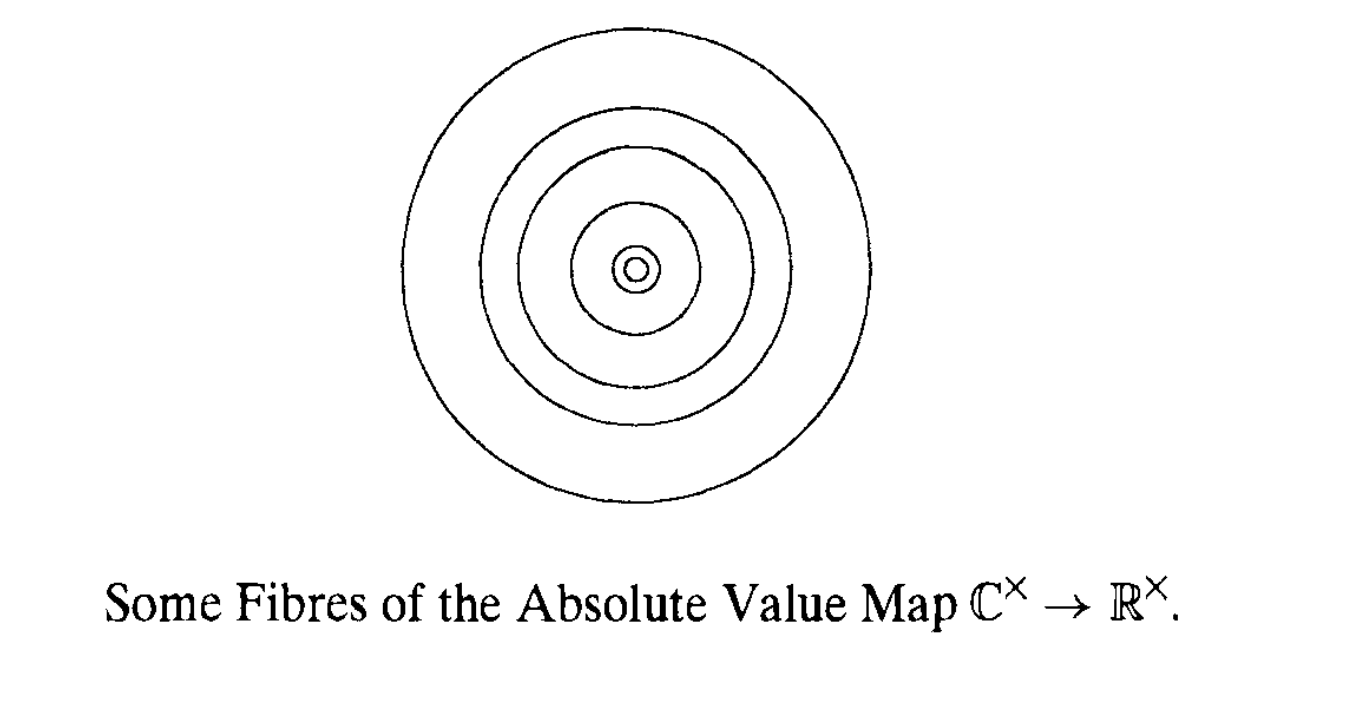
\includegraphics[width=6cm, height=3cm]{fiber.png}
\end{center}
The fibers define an equivalence relation. In other words, two elements $a, b$ are equivalent, $a\sim b$ if and only if $f(a)=f(b)$.

Let $\varphi:G\to G'$ be a homomorphism, then the fibers are given by the cosets $aK$, where $K$ is the kernel of $\varphi$.

\begin{prop}
    The order of an element $a\in G$ divides the order of the group $G$.
\end{prop}
\begin{proof}
    The order of an element $a$ is the same as the number of elements of $\langle a\rangle$, which is the cyclic group generated by $a$. By Lagrange's theorem, the order of the subgroup divides the order of the group.
\end{proof}

\begin{prop}
    Let $\varphi:G\to G'$ be a homomorphism for a finite group, then 
    \begin{equation*}
        |G|=|ker(\varphi)|\cdot |Im(\varphi)|
    \end{equation*}
\end{prop}
\begin{proof}
    This follows by cosets partition $G$ and Lagrange's theorem.
\end{proof}











\newpage

\end{document}